\section{Introducción}
\noindent En esta práctica, acidificaremos una disolución de tiosulfato (\ce{H2S2O3}) en la que precipitará azufre y enturbiará nuestras disolulciones. El fin es determinar el orden de esta reacción respecto al tiosulfato además de la velocidad inicial de reacción.\\ \\
\noindent Para ello variaremos la concentración inicial de uno de los reactivos y mantendremos las demás, analizando los datos en función de cuan rápido se produzca la reacción.

\section{Inventario}
Para esta práctica hemos usado:

\begin{itemize}
    \item 3 Buretas
    \item Tubo de ensayo
    \item Cronómetro
    \item 7 Vasos de precipitados ($100ml$)
    \item \ce{H2SO4} $0.5M$
    \item \ce{Na2S2O3} $0.3M$
    \item Frascos lavadores
\end{itemize}

\vspace{0.8cm}

\begin{figure}[H]
    \centering
    \hspace*{-3cm}
        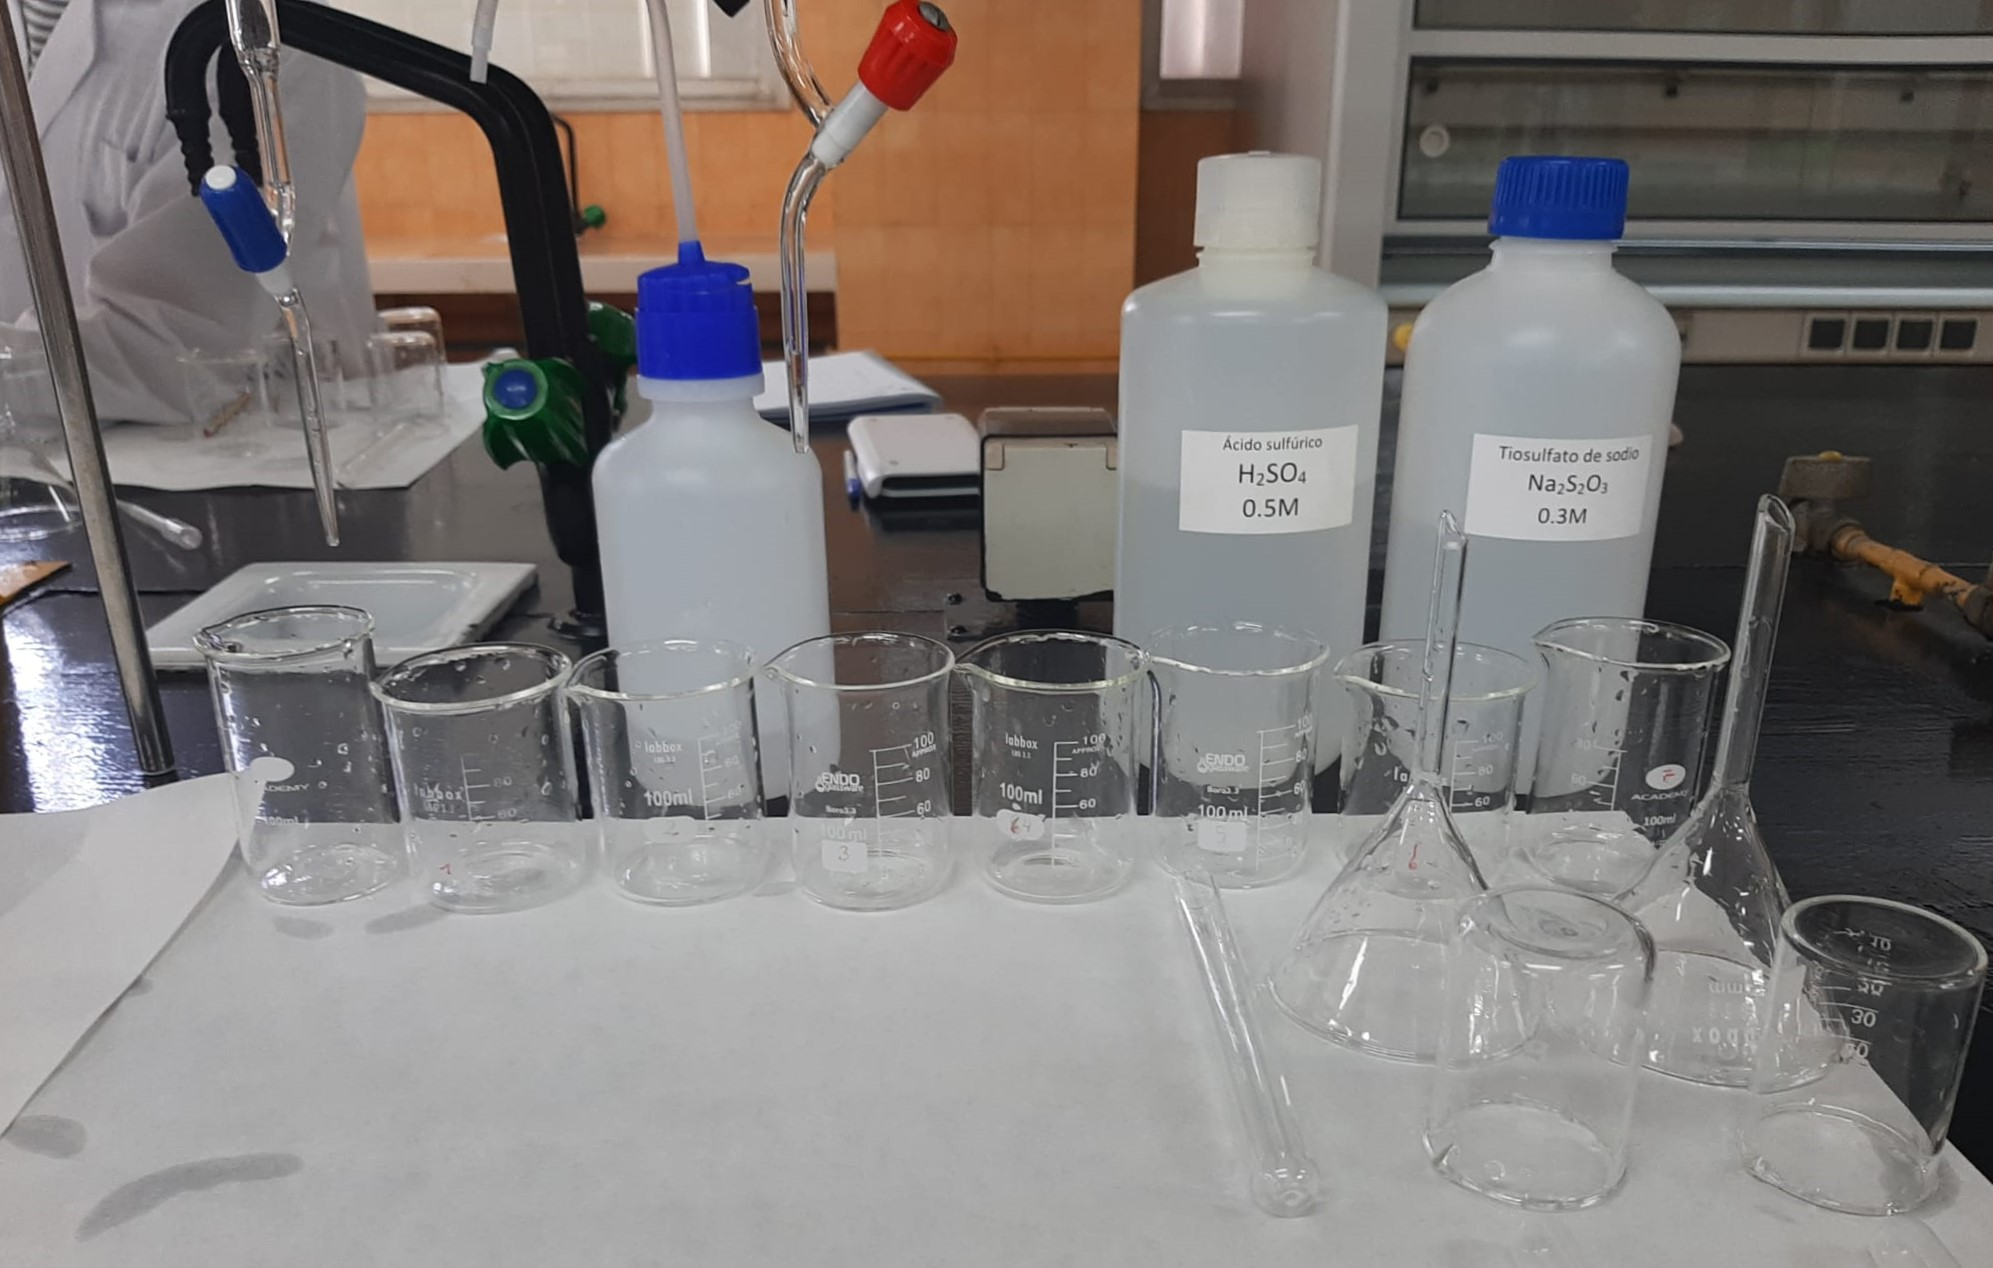
\includegraphics[scale = 0.2]{prac7/Inventario Todo.jpeg}
        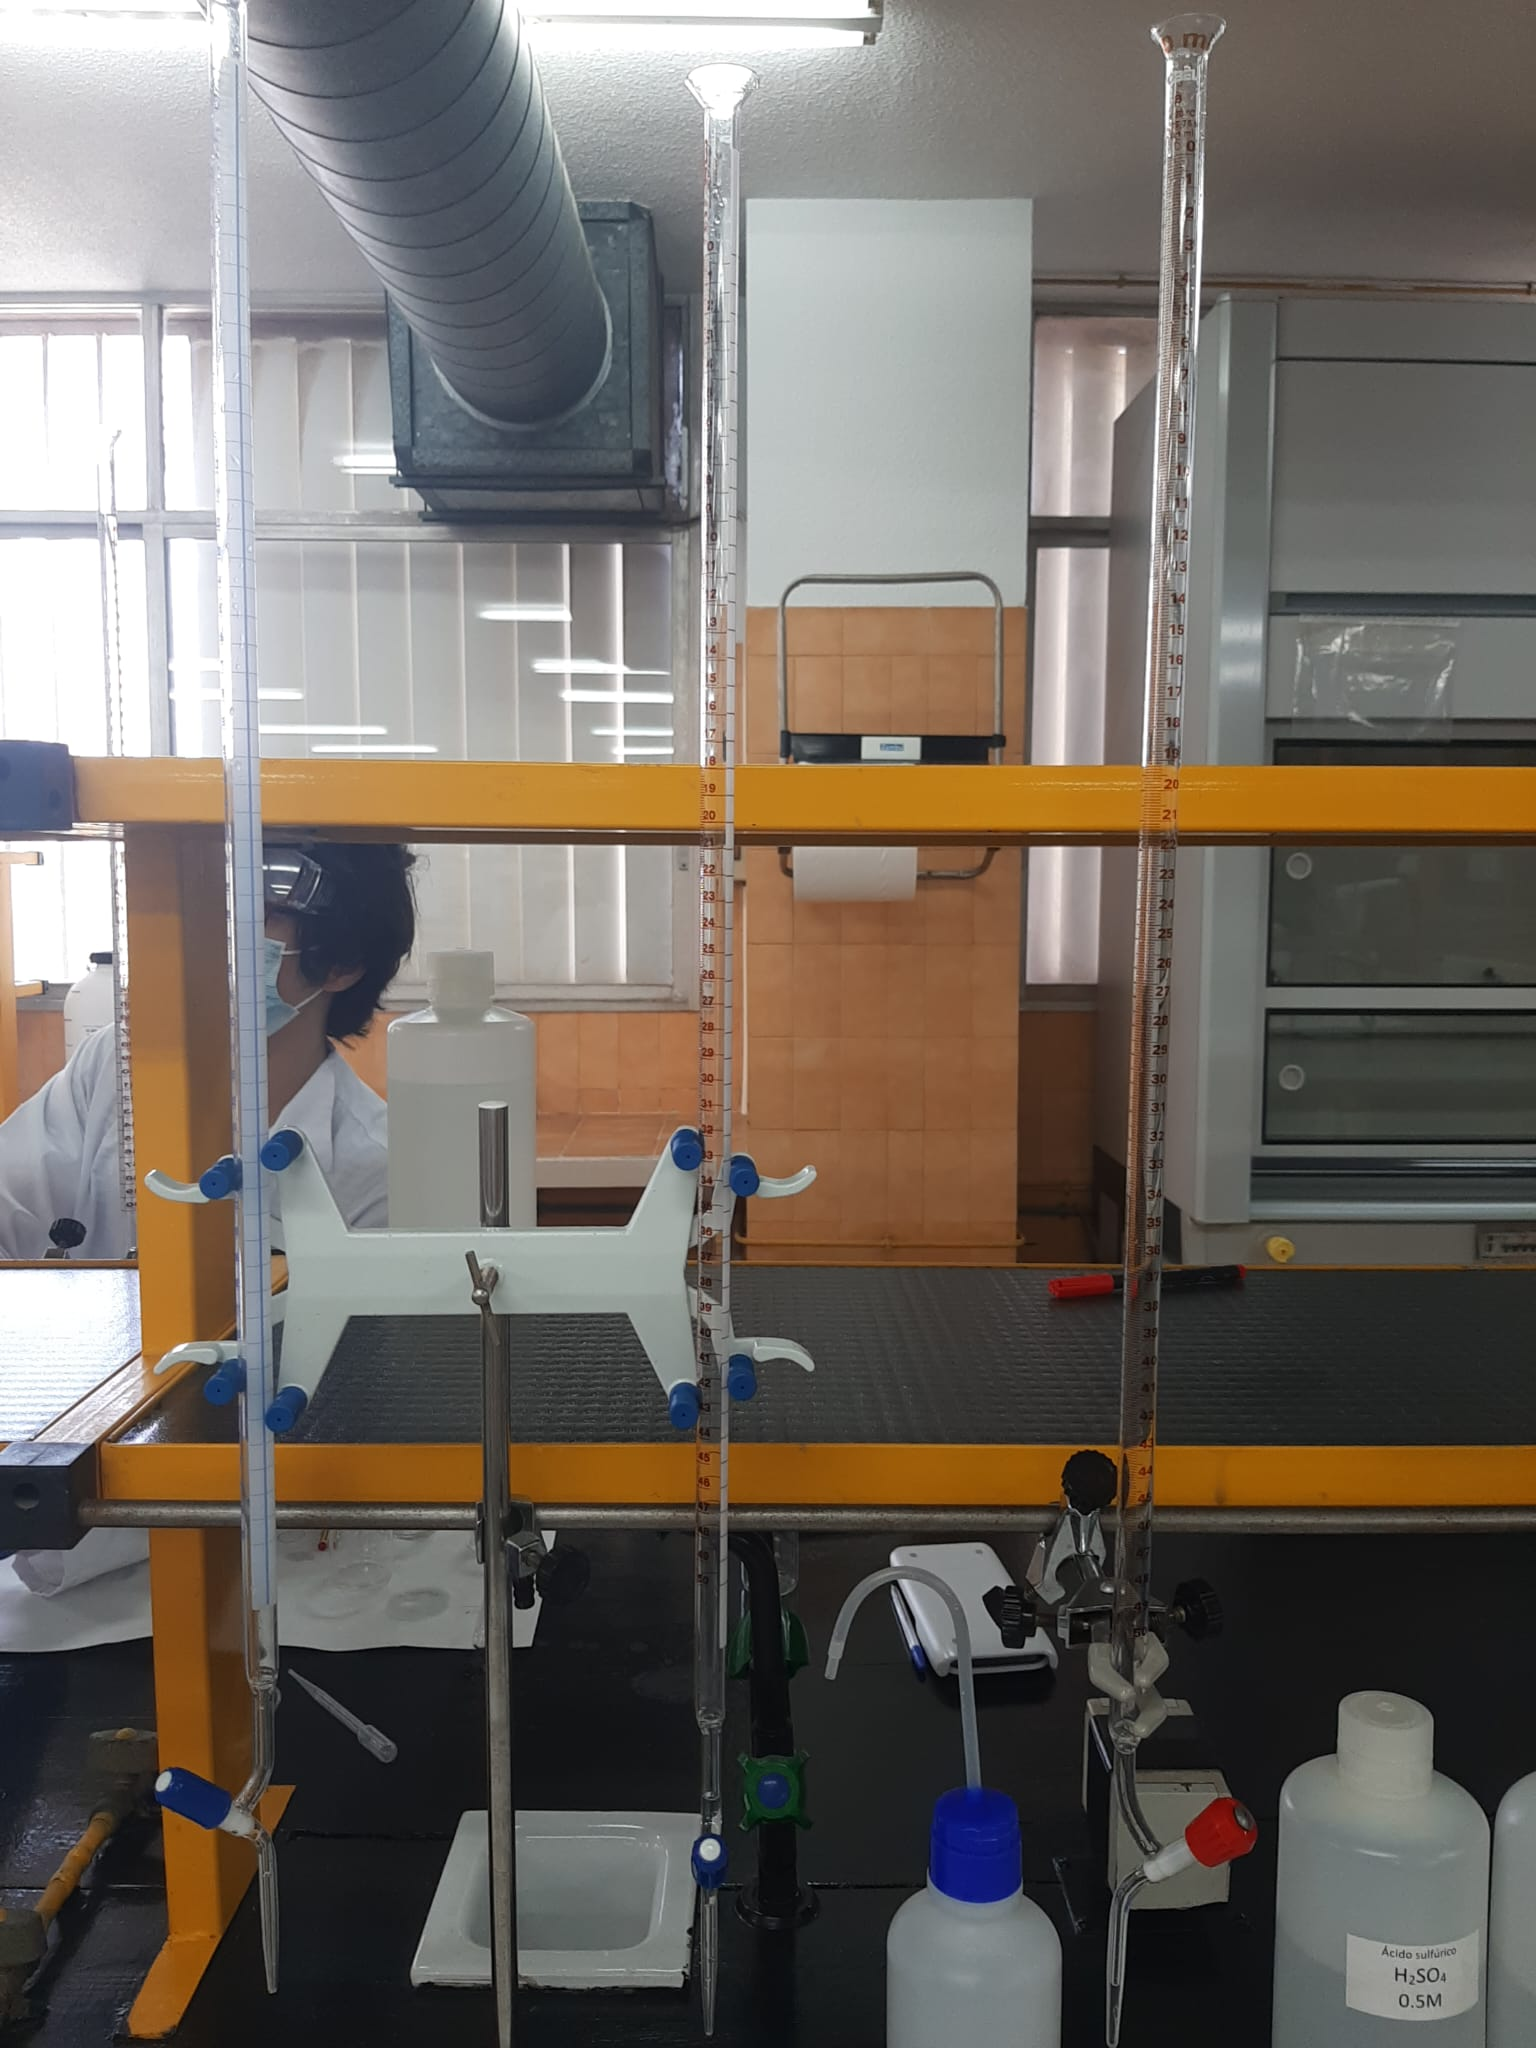
\includegraphics[scale = 0.093]{prac7/Buretas.jpeg}
    \hspace*{-3cm}
    \caption{Material utilizado a lo largo de la práctica}
    \vspace{-2cm}
\end{figure}
\clearpage

\section{Procedimiento}
\vspace{0.2cm}
\noindent Llenaremos las 3 buretas, la primera con agua destilada (\ce{H2O}), otra con ácido sulfúrico (\ce{H2SO4}) $0.5 M$ y la última con tiosulfato de sodio (\ce{Na2S2O3}) $0.3 M$. Numeraremos los vasos de precipitados que se nos dan y, ayudándonos de las buretas, llenaremos cada vaso de precipitados con las cantidades que se indican en la siguiente tabla.

\vspace{0.6cm}
\begin{table}[H]
\centering
\begin{tabular}{ccc}
\rowcolor[HTML]{CBCEFB} 
{\color[HTML]{000000} Número de Vaso} & {\color[HTML]{000000} Volúmen de \ce{Na2S2O3} ($ml$)} & {\color[HTML]{000000} Volúmen de \ce{H2O} ($ml$)} \\
\rowcolor[HTML]{ECF4FF} 
1 & 12 & 0 \\
2 & 8 & 4 \\
\rowcolor[HTML]{ECF4FF} 
3 & 6 & 6 \\
4 & 4 & 8 \\
\rowcolor[HTML]{ECF4FF} 
5 & 3 & 9 \\
6 & 2 & 10 \\
\rowcolor[HTML]{ECF4FF} 
7 & 1 & 11
\end{tabular}
\caption{volúmenes colocados en los vasos de precipitados}
\end{table}
\vspace{0.6cm}

\noindent Ahora, en un tubo de ensayo pondremos 12 $mL$ de la disolución de ácido sulfúrico (\ce{H2SO4}), que utilizaremos para verter en cada uno de los vasos, agitandolos bien y cronometrando el tiempo que esperamos hasta que empieza a aparecer turbidez. Este tiempo se anotará en una tabla, y se repetirá 3 veces el experimento para reducir el error humano del proceso.\\

\vspace{0.6cm}
\begin{table}[H]
\hspace*{-2cm}
\centering
\begin{tabular}{cccllclcc}
\cellcolor[HTML]{F6D594}{\color[HTML]{000000} Número de Vaso} &  & \cellcolor[HTML]{F6D594}Medida 1 - Tiempo ($s$) &  &  & \cellcolor[HTML]{F6D594}Medida 2 - Tiempo ($s$) &  &  & \cellcolor[HTML]{F6D594}Medida 3 - Tiempo ($s$) \\
\cellcolor[HTML]{EAEABE}1 &  & \cellcolor[HTML]{EAEABE}$8.38$ &  &  & \cellcolor[HTML]{EAEABE}$8.93$ &  &  & \cellcolor[HTML]{EAEABE}$8.80$ \\
2 &  & $12.21$ &  &  & $12.87$ &  &  & $12.13$ \\
\cellcolor[HTML]{EAEABE}3 &  & \cellcolor[HTML]{EAEABE}$17.83$ &  &  & \cellcolor[HTML]{EAEABE}$18.78$ &  &  & \cellcolor[HTML]{EAEABE}$16.34$ \\
4 &  & $24.55$ &  &  & $23.61$ &  &  & $22.26$ \\
\cellcolor[HTML]{EAEABE}5 &  & \cellcolor[HTML]{EAEABE}$31.75$ &  &  & \cellcolor[HTML]{EAEABE}$36.50$ &  &  & \cellcolor[HTML]{EAEABE}$33.59$ \\
6 &  & $52.46$ &  &  & $51.49$ &  &  & $48.53$ \\
\cellcolor[HTML]{EAEABE}7 &  & \cellcolor[HTML]{EAEABE}$108.96$ &  &  & \cellcolor[HTML]{EAEABE}$99.50$ &  &  & \cellcolor[HTML]{EAEABE}$104.06$
\end{tabular}
\caption{Resultados obtenidos a lo largo de la práctica}
\hspace*{-2cm}
\label{resultados7}
\end{table}
\clearpage

\section{Cuestiones}
\noindent\textcolor{BlueViolet}{\textbf{\textit{a) Calcule la concentración inicial de tiosulfato sódico $([A]_0)$ en cada vaso. Represente gráficamente $\log(\frac{1}{\Delta t})$ frente a $\log[A]_0$. Obtenga la ecuación de la recta a partir de la representación gráfica. Indique cuál es el orden de reacción experimental con respecto
al tiosulfato.}}}\\
\noindent Lo primero que haremos será reazliar una media de todas las medidas realizadas y descritas en el \ref{resultados7}
\begin{table}[H]
\centering
\begin{tabular}{cc}
\rowcolor[HTML]{F6D594} 
Número de Vaso & Tiempo (s) \\
\rowcolor[HTML]{EAEABE} 
1 & $08.70$ \\
2 & $12.40$ \\
\rowcolor[HTML]{EAEABE} 
3 & $17.65$ \\
4 & $23.47$ \\
\rowcolor[HTML]{EAEABE} 
5 & $33.95$ \\
6 & $50.83$ \\
\rowcolor[HTML]{EAEABE} 
\textbf{7} & $103.84$
\end{tabular}
\caption{Media de los resultados obtenidos}
\label{tab:my-table}
\end{table}
\noindent Ahora procedemos a calcular la concentración de tiosulfato sódico para cada vaso. Para hacerlo, usamos la expresión para calcular la concentración de una disolución:
\[M = \frac{\text{moles de soluto} (\si{n})}{\text{volumen de disolución} (\si{L})}\]
y por tanto,
\[\text{moles de soluto} (\si{n}) = M \cdot \text{volumen de la disolución} (\si{L})\]
\noindent Calculamos así los moles de soluto para cada vaso. Con ello y el volumen de agua añadido, calculamos la nueva concentración. Los resultados vienen representados en la tabla:
\begin{table}[H]
\centering
\begin{tabular}{ccc}
\rowcolor[HTML]{F6D594} 
Número de Vaso & Moles de soluto (\si{mol}) & Concentración (\si{M}) \\
\rowcolor[HTML]{EAEABE} 
1 & $3.6\cdot10^{-3}$ & $0.3$ \\
2 & $2.4\cdot10^{-3}$ & $0.2$ \\
\rowcolor[HTML]{EAEABE} 
3 & $1.8\cdot10^{-3}$ & $0.15$ \\
4 & $1.2\cdot10^{-3}$ & $0.1$ \\
\rowcolor[HTML]{EAEABE} 
5 & $9\cdot10^{-4}$ & $0.075$ \\
6 & $6\cdot10^{-4}$ & $0.05$ \\
\rowcolor[HTML]{EAEABE} 
7 & $3\cdot10^{-4}$ & $0.025$
\end{tabular}
\caption{Concentraciones}
\label{concentraao}
\end{table}
\clearpage

\noindent Una vez obtenidos los datos de las concentraciones inciales, vamos a representar $\log \frac{1}{\Delta \si{t}}$ frente a $\log [A]_0$ a partir de la expresión:
\[\log \frac{1}{\Delta \si{t}} = \log 1^{k'}\ - \ \log\Delta x\ +\ n_A\cdot\log [A]_0\]
\noindent Para ello primeramente calculamos los logaritmos que aparecen en la siguiente tabla:
\begin{table}[H]
\centering
\begin{tabular}{ccc}
\rowcolor[HTML]{F6D594} 
Número de Vaso & $\log \frac{1}{\Delta\si{t}}$ & $\log [A]_0$ \\
\rowcolor[HTML]{EAEABE} 
1 & $-2.16$ & $-1.20$ \\
2 & $-2.52$ & $-1.60$ \\
\rowcolor[HTML]{EAEABE} 
3 & $-2.87$ & $-1.90$ \\
4 & $-3.16$ & $-2.30$ \\
\rowcolor[HTML]{EAEABE} 
5 & $-3.52$ & $-2.59$ \\
6 & $-3.93$ & $-2.99$ \\
\rowcolor[HTML]{EAEABE} 
7 & $-4.64$ & $-3.69$
\end{tabular}
\caption{Logaritmos}
\label{logaritmos}
\end{table}

\begin{figure}[H]
    \centering
    \hspace*{-3cm}
        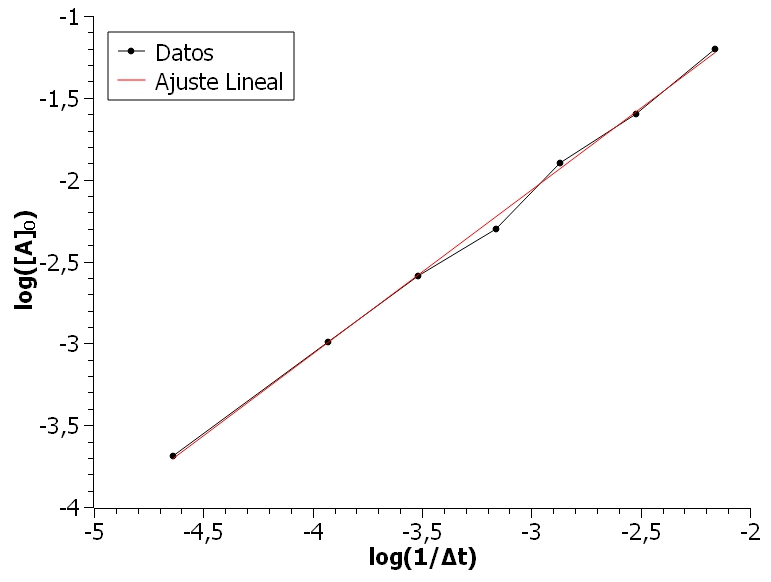
\includegraphics[scale = 0.5]{prac7/logaritmos.jpg}
    \hspace*{-3cm}
    \caption{Representación Gráfica}
\end{figure}

\noindent Del ajuste lineal obtenemos una ordenada en el origen de 0.93, siendo 1 el número natural más cercano y, por tanto, siendo 1 el orden de la reacción. La ecuación de la recta obtenida es $y = ax+b$, siendo $a = 1$ y $b = 0.93$.